\documentclass[11pt,twoside,a4paper,openright]{report}
%synctex =====EXPERIMENTAL======
\synctex=1

% Select encoding of your inputs
\usepackage[utf8]{inputenc}

% Make latex understand and use the typographic
% rules of the language used in the document.
\usepackage[english]{babel}

% Use the vector font Latin Modern which is going
% to be the default font in latex in the future.
\usepackage{lmodern}

% Choose the font encoding
\usepackage[T1]{fontenc}

% Use color in tables
\usepackage[table]{xcolor}
\usepackage{array}
\usepackage{multirow}

% Load a colour package
\usepackage{xcolor}
\definecolor{aaublue}{RGB}{33,26,82}  %<--define aaublue
\definecolor{white}{RGB}{255,255,255} %<--define white

% The standard graphics inclusion package
\usepackage{graphicx}

\makeatletter
  \g@addto@macro\@floatboxreset\centering %<--centering all figures
\makeatother

\usepackage{adjustbox}

% Set up how figure and table captions are displayed
\usepackage{float}
\usepackage{caption}
\usepackage{subcaption}
\setlength{\belowcaptionskip}{-0.5cm}
\captionsetup
{
  justification = centering,    %<--centering caption with multiple lines
  font          = footnotesize, %<--set font size to footnotesize
  labelfont     = bf            %<--bold label (e.g., Figure 3.2) font
}
\captionsetup[subfigure]
{
  justification = centering, %<--centering subfigure caption text
  singlelinecheck=false,
  font = footnotesize        %<--font size for subfigures
} 

% Enable row combination in tables
\usepackage{multirow}

% Make space between table lines and text
\renewcommand{\arraystretch}{1.5}

% Enable commands like \st (strike out) and \hl (high light)
\usepackage{soul}

% Make the standard latex tables look so much better
\usepackage{array,booktabs}

% Enable the use of frames around, e.g., theorems
% The framed package is used in the example environment
\usepackage{framed}
\usepackage{colortbl}
\usepackage{longtable}
\usepackage{xcolor}
\usepackage{textcomp}

%-------MATHEMATICS---------------------------------
% Defines new environments such as equation,
% align and split 
\usepackage{amsmath}
\usepackage{mathtools}
\usepackage{relsize}
% Adds new math symbols
\usepackage{amssymb}
% Use theorems in your document
% The ntheorem package is also used for the example environment
% When using thmmarks, amsmath must be an option as well. Otherwise \eqref doesn't work anymore.
\usepackage[framed,amsmath,thmmarks]{ntheorem}
\usepackage{xifthen}%<--enables ifthenelse which is used in macros

\usepackage{siunitx} 
\sisetup{decimalsymbol=period}%<--\num{} will swich commas with periods
\sisetup{detect-weight}
%---------------------------------------------------

%-------PAGE LAYOUT---------------------------------
% Change margins, papersize, etc of the document
\usepackage[
  left=25mm,% left margin on an odd page %tidligere 25mm for baade right og left
  right=25mm,% right margin on an odd page
  top=35mm,
  ]{geometry}
  
% Modify how \chapter, \section, etc. look
% The titlesec package is very configureable
\usepackage{titlesec}
\makeatletter
\def\ttl@mkchap@i#1#2#3#4#5#6#7{%
    \ttl@assign\@tempskipa#3\relax\beforetitleunit
    \vspace{\@tempskipa}%<<<<<< REMOVE THE * AFTER \vspace
    \global\@afterindenttrue
    \ifcase#5 \global\@afterindentfalse\fi
    \ttl@assign\@tempskipb#4\relax\aftertitleunit
    \ttl@topmode{\@tempskipb}{%
        \ttl@select{#6}{#1}{#2}{#7}}%
    \ttl@finmarks  % Outside the box!
    \@ifundefined{ttlp@#6}{}{\ttlp@write{#6}}}
\makeatother

\titlespacing{\chapter}{0pt}{0pt}{10pt}
\titlespacing{\section}{0pt}{0pt}{-5pt}
\titlespacing{\subsection}{0pt}{8pt}{-5pt}
\titlespacing{\subsubsection}{0pt}{6pt}{-10pt}

\titleformat*{\section}{\normalfont\Large\bfseries\color{aaublue}}
\titleformat*{\subsection}{\normalfont\large\bfseries\color{aaublue}}
\titleformat*{\subsubsection}{\normalfont\normalsize\bfseries\color{aaublue}}

\usepackage{titlesec, blindtext, color}
%\color{gray75}{gray}{0.75}
\newcommand{\hsp}{\hspace{20pt}}
\titleformat{\chapter}[hang]{\Huge\bfseries}{\thechapter\hsp\textcolor{aaublue}{|}\hsp}{0pt}{\Huge\bfseries}

% Change the headers and footers
\usepackage{fancyhdr}
\setlength{\headheight}{15pt}
\pagestyle{fancy}
\fancyhf{} %delete everything
\renewcommand{\headrulewidth}{0pt} %remove the horizontal line in the header
\fancyhead[RO,LE]{\color{aaublue}\small\nouppercase\leftmark} %even page - chapter title
\fancyhead[LO]{}
\fancyhead[RE]{} 
\fancyhead[CE]{}
\fancyhead[CO]{}
\fancyfoot[RE,LO]{\thepage}
\fancyfoot[LE,RO]{} %page number on all pages
\fancyfoot[CE,CO]{}

% change first page of all chapters header and footer to fancy style
\makeatletter
\let\ps@plain\ps@fancy
\makeatother

% Do not stretch the content of a page. Instead,
% insert white space at the bottom of the page
\raggedbottom

% Enable arithmetics with length. Useful when typesetting the layout.
\usepackage{calc}
%---------------------------------------------------

%-------BIBLIOGRAPHY--------------------------------
%setting references (using numbers) and supporting i.a. Chicargo-style:
\usepackage{etex}
\usepackage{etoolbox}
\usepackage{keyval}
\usepackage{ifthen}
\usepackage{url}
\usepackage{csquotes}
\usepackage[backend=biber, url=true, urldate=long, doi=true, style=numeric, sorting=none]{biblatex}
\addbibresource{setup/bibliography.bib}
%---------------------------------------------------

%-------MISC----------------------------------------
%%% Enables the use FiXme refferences. Syntax: \fxnote{...} %%%
\usepackage[footnote, draft, english, silent, nomargin]{fixme}
%With "final" instead of "draft" an error will ocure for every FiXme under compilation.

%%% allows use of lorem ipsum (generate i.e. pagagraph 1 to 5 with \lipsum[1-5]) %%%
\usepackage{lipsum}

%%% Enables figures with text wrapped tightly around it %%%
\usepackage{wrapfig}

%%% Section debth included in table of contents (1 = down to sections) %%%
\setcounter{tocdepth}{1}

%%% Section debth for numbers (1 = down to sections) %%%
\setcounter{secnumdepth}{2}

\usepackage{tocloft}
\setlength{\cftbeforetoctitleskip}{0 cm}
\renewcommand{\cftpartpresnum}{Part~}
\let\cftoldpartfont\cftpartfont
\renewcommand{\cftpartfont}{\cftoldpartfont\cftpartpresnum}
%---------------------------------------------------

%-------HYPERLINKS----------------------------------
% Enable hyperlinks and insert info into the pdf
% file. Hypperref should be loaded as one of the 
% last packages
\usepackage{nameref}
\usepackage{hyperref}
\usepackage{bookmark}
\hypersetup{%
	%pdfpagelabels=true,%
	plainpages=false,%
	pdfauthor={Author(s)},%
	pdftitle={Title},%
	pdfsubject={Subject},%
	bookmarksnumbered=true,%
	colorlinks,%
	citecolor=aaublue,%
	filecolor=aaublue,%
	linkcolor=aaublue,% you should probably change this to black before printing
	urlcolor=aaublue,%
	pdfstartview=FitH%
}
%---------------------------------------------------

% remove all indentations
\setlength\parindent{0pt}
\parskip 5mm
\usepackage{verbatim}

\definecolor{Gra}{RGB}{230,230,230}

%creates a nice-looking C#-text
\newcommand{\CC}{C\nolinebreak\hspace{-.05em}\raisebox{.3ex}{\scriptsize\text \#} }

%enables multi column lists
\usepackage{multicol}

%enables code-examples
\usepackage{listings}

\definecolor{coolblue}{RGB}{32,95,128}
\definecolor{mygreen}{rgb}{0,0.6,0}
\definecolor{mygray}{rgb}{0.5,0.5,0.5}
\definecolor{mymauve}{rgb}{0.58,0,0.82}
\usepackage{textcomp}
\definecolor{listinggray}{gray}{0.9}
\definecolor{lbcolor}{rgb}{0.9,0.9,0.9}

%for c code
\lstdefinestyle{cstyle}{
  backgroundcolor=\color{lbcolor},
	tabsize=4,
	rulecolor=,
	language=C,
  basicstyle=\scriptsize,
  upquote=true,
  aboveskip={1.5\baselineskip},
  columns=fixed,
  showstringspaces=false,
  extendedchars=true,
  breaklines=true,
  prebreak = \raisebox{0ex}[0ex][0ex]{\ensuremath{\hookleftarrow}},
  frame=single,
  showtabs=false,
  numbers=left,
  captionpos=b,
  numbersep=5pt,
  numberstyle=\tiny\color{mygray},
  showspaces=false,
  showstringspaces=false,
  identifierstyle=\ttfamily,
  keywordstyle=\color[rgb]{0,0,1},
  commentstyle=\color[rgb]{0.133,0.545,0.133},
  stringstyle=\color[rgb]{0.627,0.126,0.941},
}
%for python code
\lstdefinestyle{pythonstyle}{
    backgroundcolor=\color{lbcolor},
    tabsize=4,
    rulecolor=,
    language=python,
    basicstyle=\scriptsize,
    upquote=true,
    aboveskip={1.5\baselineskip},
    columns=fixed,
    showstringspaces=false,
    extendedchars=true,
    breaklines=true,
    prebreak = \raisebox{0ex}[0ex][0ex]{\ensuremath{\hookleftarrow}},
    frame=single,
    showtabs=false,
    numbers=left,
    captionpos=b,
    numbersep=5pt,
    numberstyle=\tiny\color{mygray},
    showspaces=false,
    showstringspaces=false,
    identifierstyle=\ttfamily,
    keywordstyle=\color[rgb]{0,0,1},
    commentstyle=\color[rgb]{0.133,0.545,0.133},
    stringstyle=\color[rgb]{0.627,0.126,0.941},
}
%for matlab code
\lstdefinestyle{matlabstyle}{
    backgroundcolor=\color{lbcolor},
    tabsize=4,
    rulecolor=,
    language=Matlab,
    basicstyle=\scriptsize,
    upquote=true,
    aboveskip={1.5\baselineskip},
    columns=fixed,
    showstringspaces=false,
    extendedchars=true,
    breaklines=true,
    prebreak = \raisebox{0ex}[0ex][0ex]{\ensuremath{\hookleftarrow}},
    frame=single,
    showtabs=false,
    numbers=left,
    captionpos=b,
    numbersep=5pt,
    numberstyle=\tiny\color{mygray},
    showspaces=false,
    showstringspaces=false,
    identifierstyle=\ttfamily,
    keywordstyle=\color[rgb]{0,0,1},
    commentstyle=\color[rgb]{0.133,0.545,0.133},
    stringstyle=\color[rgb]{0.627,0.126,0.941},   
}
%for inline c, syntax: \cline{ codeHere(); }
\lstdefinestyle{cinline}{
    style=cstyle,
    basicstyle=\small,
}
\newcommand\inlinec[1]{ \lstinline[style=cinline]{#1} }

%for inline python, syntax: \pythonline{ codeHere(); }
\lstdefinestyle{pythoninline}{
    style=pythonstyle,
    basicstyle=\small,
}
\newcommand\inlinepython[1]{ \lstinline[style=pythoninline]{#1} }

%for inline matlab, syntax: \matlabline{ codeHere(); }
\lstdefinestyle{matlabinline}{
    style=matlabstyle,
    basicstyle=\small,
}
\newcommand\inlinematlab[1]{ \lstinline[style=matlabinline]{#1} }

\usepackage{enumitem}
%\usepackage[citestyle=authoryear,natbib=true]{biblatex}

% Figures - TIKZ
\usepackage{tikz}
\usepackage[americanresistors,americaninductors,americancurrents, americanvoltages]{circuitikz}

% Wall of text logo
\newcommand{\walloftextalert}[0]{\includegraphics[width=\textwidth]{walloftext.png}}

\usepackage{pdfpages}
\usepackage{lastpage}
\usepackage{epstopdf}

\setlength{\headheight}{21pt}

\hfuzz=\maxdimen
\tolerance = 10000
\hbadness  = 10000

\usepackage{siunitx}
\graphicspath{{./figures/}}
% package inclusion and set up of the document

%Macro for 'where'-enviroment was improved by Andrea and Niels :-)

%-----------UNITS-------------------------------------------
\newcommand{\unit}[1]{&& \left[\si{#1}\right]}
%
%\newcommand{\unit}[1]{[\si{#1}]}            %<<| Use these if you want equations to be
%\newcommand{\eq}[2]{&&\si{#1} &= \si{#2}&&} %<<| centered.. .. will appear scrambled
%                                            %  | from one equation to the next though..
%                                            %  | and does not work with long equations.. :/
%
%-----------------------------------------------------------

%-----------WHERE ENVIRONMENT-------------------------------
\newenvironment{where}{\leavevmode{\parindent=1em\indent} Where:\\}{}
\newcommand{\va}[3]
{
  \begin{tabular}{p{20pt} p{40pt} p{290pt} l}
    & { $#1$ } & { #2 } & \ifthenelse{\isempty{ #3 }}  {}  {[{\si{#3}}]} \\
  \end{tabular}\\
}
%-----------------------------------------------------------

%-----------TikZ SETTINGS-----------------------------------
\tikzset{
  block/.style    = {draw, thick, rectangle,
                     minimum height = 2.1em,
                     minimum width = 1.7em},
  sum/.style      = {draw, circle, inner sep=3pt} %<--Adder
}
%-----------------------------------------------------------% my new macros

\begin{document}
    %%% Prereport %%%
    \setlength\cftaftertoctitleskip{2pt}
    \setlength\cftafterloftitleskip{6pt}
    \setlength\cftafterlottitleskip{6pt}
    \selectlanguage{english}
    \title{Vessel}
    
    %%% Frontmatter Settings %%%
    \pagestyle{empty} %disable headers and footers
    \pagenumbering{roman} %use roman page numbering in the frontmatter I II...
    \fancyfoot[RE,LO]{17gr832} %page number on all pages
    \fancyfoot[LE,RO]{\thepage}
    \fancyhead[LE,LO,RE,RO]{}
    
    %%% Introductory Formalities %%%
    %\includepdf[pages={1}]{formalities/frontpage.pdf}
    \pdfbookmark[0]{Front Page}{label:forside}%
\begin{titlepage}
    \addtolength{\hoffset}{0.5\evensidemargin-0.5\oddsidemargin} %set equal margins on the frontpage - remove this line if you want default margins
    \noindent%
    \begin{tabular}{@{}p{\textwidth}@{}}
        \toprule[2pt]
        \midrule
        \vspace{0.2cm}
        \begin{center}
            \Huge{\textbf{Precision Control of an Autonomous\\ Surface Vessel}}
        \end{center}
    	\vspace{0.19cm} \\
        \midrule
        \toprule[2pt]
    \end{tabular}
    \centering
    \vspace{1.7 cm}
    \begin{figure}[!ht]
        \centering
        \includegraphics[width=0.8\textwidth]{figures/frontpage}
        \label{fig:forside}
    \end{figure}
    \vspace{1.7 cm}
    \begin{center}
        {\large 
        2$^{\mathrm{nd}}$ Semester Master's Program in Control and Automation\\
        Department of Electronic Systems\\
        Aalborg University \\
        }
        \vspace{1cm}
        { 
        Alejandro Alonso García, Anders Egelund Kjeldal, Himal Kooverjee, \\ Niels Skov Vestergaard and Noelia Villarmarzo Arruñada \\
        Group 832
        }
    \end{center}
    \vspace{-0.5 cm}
\end{titlepage}
\clearpage
    \pagestyle{fancy}
    {\small
\strut\vfill % push the content to the bottom of the page
\noindent Copyright \copyright{} Aalborg University 2017\par
\vspace{0.2cm}

\noindent This report is compiled in \LaTeX, originally developed by Leslie Lamport, based on Donald Knuth's \TeX. The main text is written in \emph{Latin Modern} pt 12, designed by Bogusław Jackowski and Janusz M. Nowacki. 
%The document is compiled via the website \url{www.overleaf.com}, an online collaborative based \LaTeX-editor with instant preview, which enables multiple persons to edit the document simultaneously.
Flowcharts and diagrams are made using Inkscape. 
\clearpage
    %\begin{document} 
%\thispagestyle{empty}
%\begin{titlepage}
\begin{nopagebreak}
{\samepage 

\begin{tabular}{r}
\parbox{\textwidth}{  \raisebox{-15mm}{
\includegraphics[height=3cm]{figures/aaulogo-en.png}}
\hfill \hspace{2cm} \parbox{8cm}{\begin{tabular}{l} %4.90
{\small \textbf{\textcolor{black}{\colorbox{white}{2\textsuperscript{nd} Semester Project}}}}\\
{\small \textbf{\textcolor{black}{Master's Program in}}}\\ 
{\small \textbf{\textcolor{black}{Control and Automation}}}\\ 
{\small \textcolor{black}{Department of Electronic Systems}}\\
{\small \textcolor{black}{Fredrik Bajers Vej 7C, 9220 Aalborg}} \\
 \\
%{\small \textcolor{black}{\emph{http://www.sict.aau.dk/electronics-and-it}}}
\end{tabular}}}
\end{tabular}

\begin{tabular}{cc}
\parbox{7cm}{

\textbf{Title:} \\
Precision Control of an Autonomous Surface Vessel \\

\textbf{Theme:} \\
\small{Multivariable Control
\\
}

\parbox{8cm}{

\textbf{Project Period:}\\
Spring 2017\\
%01/09/2016 - 20/12/2016\\
   
\textbf{Project Group:}\\
832\\ %\fxnote{Input group number}
  
\textbf{Participants:}\\
Alejandro Alonso García\\
Anders Egelund Kjeldal\\
Himal Kooverjee  \\
Niels Skov Vestergaard\\
Noelia Villarmarzo Arruñada\\

\textbf{Supervisor:}\\Jesper Abildgaard Larsen\\
}

\textbf{Pages:} 106 \\ 
\textbf{Appendices:} 10 \\
\textbf{Attachments:} 1 \\

\textbf{Concluded:} 30/06/2017\\

\vfill } &
\parbox{7cm}{
  \vspace{.15cm}
  \hfill
  \begin{tabular}{l}
  {\textbf{Synopsis:}} \\
  \fbox{
    \parbox{6.5cm}{\bigskip
     {\vfill{\small \lipsum[1-1]\fxnote{Write synopsis}
     \bigskip}}
     }}
   \end{tabular}}
\end{tabular} %\vspace{1cm}
}


\textit{\phantom{A}Publication of this report's contents (including citation) without permission\\ \phantom{A}from the authors is prohibited}\\

\end{nopagebreak}
%\end{titlepage}
%\end{document}
    %%% Preface %%%
    %\cleardoublepage
    \chapter*{Preface}
\vspace{-12 pt}
The focus of this project is to design a control system for an autonomous surface vessel, such that it can navigate autonomously over a predetermined area in the water.

This report has been written by a group of students on the second semester of the Master in Control and Automation at Aalborg University in the spring semester of 2017. It has been supervised by Jesper Abildgaard Larsen, associate professor at the Institute of Electronic Systems at Aalborg University. 

The group would like to thank Jens Frederik Dalsgaard Nielsen for his guidance during the setup of the GPS, and Palle Andersen for his help in the robust control design, both associate professors at the Institute of Electronic Systems Aalborg University.

The reader is expected to have a basic knowledge within physics and mathematics, as well as in modeling and linear control theory.

\textbf{Reading Instructions}
\vspace{-10 pt}
\begin{itemize}
    \item[-] The report is divided in three parts. Part I deals with the analysis of the system, which includes a description of the setup and the derivation of the dynamic model. Part II includes the control design, which contains the two approaches for an inner controller, the outer controller, the sensor fusion and the implementation. Part III includes the results of the project, the discussion and the conclusion.
    \item[-] The report also includes appendixes that contain the journals for the different tests and other relevant information.
    \item[-] The bibliography is written using ISO 690, noted as [x], and it is included at the end of the report, after the appendixes.
    \item[-] An attachment is included as part of the report, and contains MATLAB scripts and simulations files, test data files and the ROS workspace files used in the project.
\end{itemize}

%
\textbf{Text by:}\\
\vspace{-12 pt}
\begin{table}[H]
	\centering
		\begin{tabular}{c c c}
			\underline{\phantom{JAERJAERJAERJAERGO}} & \phantom{cookies} & \underline{\phantom{JAERJAERJAERJAERGO}} \\
			Alejandro Alonso García & \phantom{cookies} & Anders Egelund Kjeldal \\
			&&\\
			\underline{\phantom{JAERJAERJAERJAERGO}} & \phantom{cookies} & \underline{\phantom{JAERJAERJAERJAERGO}} \\
			Himal Kooverjee & \phantom{cookies} & Niels Skov Vestergaard		\\
			&&\\
	    \multicolumn{3}{c}{\underline{\phantom{JAERJAERJAERJAERGO}}}\\
	    \multicolumn{3}{c}{Noelia Villarmarzo Arruñada}\\				
		\end{tabular}
\end{table}
\pagebreak
    
    \pdfbookmark[0]{Table of Contents}{label: tableOfCentents}
    \tableofcontents
    \cleardoublepage
    
    %%% Mainmatter Settings %%%
    \pagenumbering{arabic} %use arabic page numbering in the mainmatter
    \fancyfoot[RO,LE]{\thepage \text{ of} \pageref{LastPage}}
    \fancyfoot[RE,LO]{17gr832}
    \fancyhead[RE,LO]{}
    \fancyhead[RE,LO]{\color{aaublue}\small\nouppercase\leftmark} %even page - chapter title
    \pagestyle{fancy}
    
    
    %%% PART 1 %%%
    \part{Preanalysis}
    
    %---------- Chapter 1 ---------------------------------------- Introduction
    \chapter{Introduction}

Autonomous surface vehicles (ASV) has a range of applications such as environmental monitoring \cite[p. 745]{MAHsieh}, meteorological data collection, marine biological research and surveillance \cite[p. 8-10]{FFahimi}.
The design of an ASV raises some interesting control challenges, varying between the intended use case.

One such use case is shown in \autoref{fig:USVforRescue}. 
This is an ASV designed to aid with search and rescue missions in floods. 
It can be dangerous and difficult for rescuers to search in flooded areas. 
A drone is able to reach otherwise inaccessible places and provides better vision horizons than an ASV would. 
The drone however has short battery life, which limits the reach and duration of the mission.
%
\begin{figure}[H]
  \vspace{3mm}
  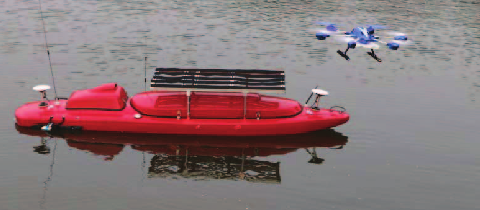
\includegraphics[width=0.62\textwidth]{figures/USVforRescue.pdf}
  \caption{An air-surface system for search in flooded areas under search and rescue missions.\cite{JZhang}}
  \label{fig:USVforRescue}
\end{figure}
\vspace{-6mm}
%
Here the ASV provides long battery life and by carrying the drone, until needed for improved overview, extends reach and duration of each mission.\cite{JZhang}


%%%%%%%%%%Survey%%%%%%%%%%

Another application is for automated survey of an area.
Bathymetric measurements can be used for efficient and safe guidance of marine vessels in shallow waters. 
It is also interesting when studying biological oceanography where it i.e. can help in deciding which areas to protect for preservation of sea life \cite{NOService}. 

%For some types of survey it is required for the ASV to maintain its GPS position while preforming measurements. 
%This requires the system to be able to estimate and counteract external forces, applied to the vessel, keeping it still. 

%A basic functionality of a ASV is to follow a route. 
%This enables to ASV to arrive at a survey side and to preform measurements along a path. 
%%%% https://pdfs.semanticscholar.org/ce94/01a72e78b314f5d2fbbce66f56b217acef1c.pdf
In volcanic countries observations are carried out by volcanologists to provide forecasts and warnings. One observation target is crater lakes. Flash floods and hydrovolcanic explosions can be caused by such lakes. Observing these can help providing information when precautions must be taken and potential evacuation planned.\cite{AWatanabe}
%
\begin{figure}[H]
  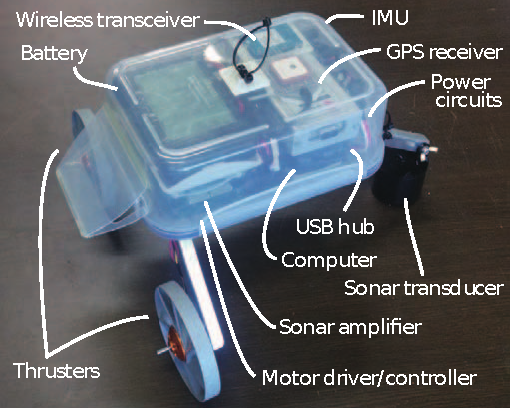
\includegraphics[width=0.35\textwidth]{figures/volcanicLakeUSVwLabels.pdf}
  \caption{Small ASV for taking bathymetric measurements in the Mt. Zao Okama Crater Lake in Japan.\cite{AWatanabe}}
  \label{fig:volcanicLakeUSVwLabels}
\end{figure}
\vspace{-6mm}
%
The small ASV seen in \autoref{fig:volcanicLakeUSVwLabels} is designed to take bathymetric measurements of such lakes and eliminate the need to endanger humans in the process.\cite{AWatanabe}

The USV is made specifically for the Mt. Zao Okama Crater Lake in Japan, where it replaces the need for a manned canoe to enter the volcanic lake situated in high
altitude, strong wind, and restricted area. The bathymetric measurements are used to indicate the amount of water, crater wall caving, and volcanic upthrusts in the lake.\cite{AWatanabe}

An example of a system designed to preform such a task is described in \cite{asv_solar}.
%This implementation achieves such functionality is through a two layer design. 
%An inner controller manipulates the dynamics of the system, while an outer controller is responsible for steering the route through the inner controller. 
This system is able to detect and avoid obstacles in the water, while preforming precision measurements of water quality and greenhouse gases. 
The vessel uses solar cells, which gives the added challenge of controlling the vessel at low speeds, to prevent battery usage during operation for longevity. 
This allows the vessel to autonomously survey relatively large areas without needing to recharge. 

%
%one strength of an ASV is that it can map out an entire stream, whereas manual measurements typicaly will be cumbersome and low in mapping resolution due to accessibility of the stream and time constraints/cost.\\
%for marine survey it can be useful as it can enter narrower and more shallow waters than larger manned vessels would be able to.\\
%the military has also been using ASV's for surveillance.
In this project, the design and implementation of an ASV able to preform bathymetric measurement will be described. 
This will be done using the aauship platform supplied for this project by Aalborg university. 
%In this project the focus is first and foremost the control design, which will be realized with focus on bathymetric measurements. This will constitute a basis for setting up requirements for precision which will determine important parameters in the control design.

    
    \chapter{Problem Analysis}
This chapter analyses the scope of the project as well as the requirements that need to be fulfilled.

\section{Scope of the Project}
The goal of this project is to develop a control strategy that can make the autonomous surface vessel be suitable for survey tasks in the water. More specifically, it should be able to perform bathymetric measurements.

The controller design must be able to track references provided by the trajectory planer as well as rejecting disturbances such as possible wind or the effect of the waves. This requires to include a model of the disturbances in the controller design as well as a robust controller capable of handling model uncertainties.

The trajectory planer needs to be able to design a route in the form of waypoints, to send to the controller, to reach all the position needed to perform the different measurements required for the survey. 

One important aspect to be taken into account is the precision of the route tracking, that should be below 10 cm. This requires a positioning system able of providing position data with more precision that the GPS module mounted on the vessel. A test that shows the distribution of the sample from this GPS can be seen in \fxnote{Refer to test with GPS to show it is not enough} For that reason, an RTK GPS is more suitable to enhance the precision of position data.


\section{Requirements} \label{sec:requirements}
To be able to design a working product some functional requirements need to be set and verified at the end of the project once all the design has been carried out.

- tracking of reference position with a precision below 10 cm

- 

    %---------- Chapter 2 ---------------------------------------- System Description
    \chapter{System Description}

\begin{figure}[H]
    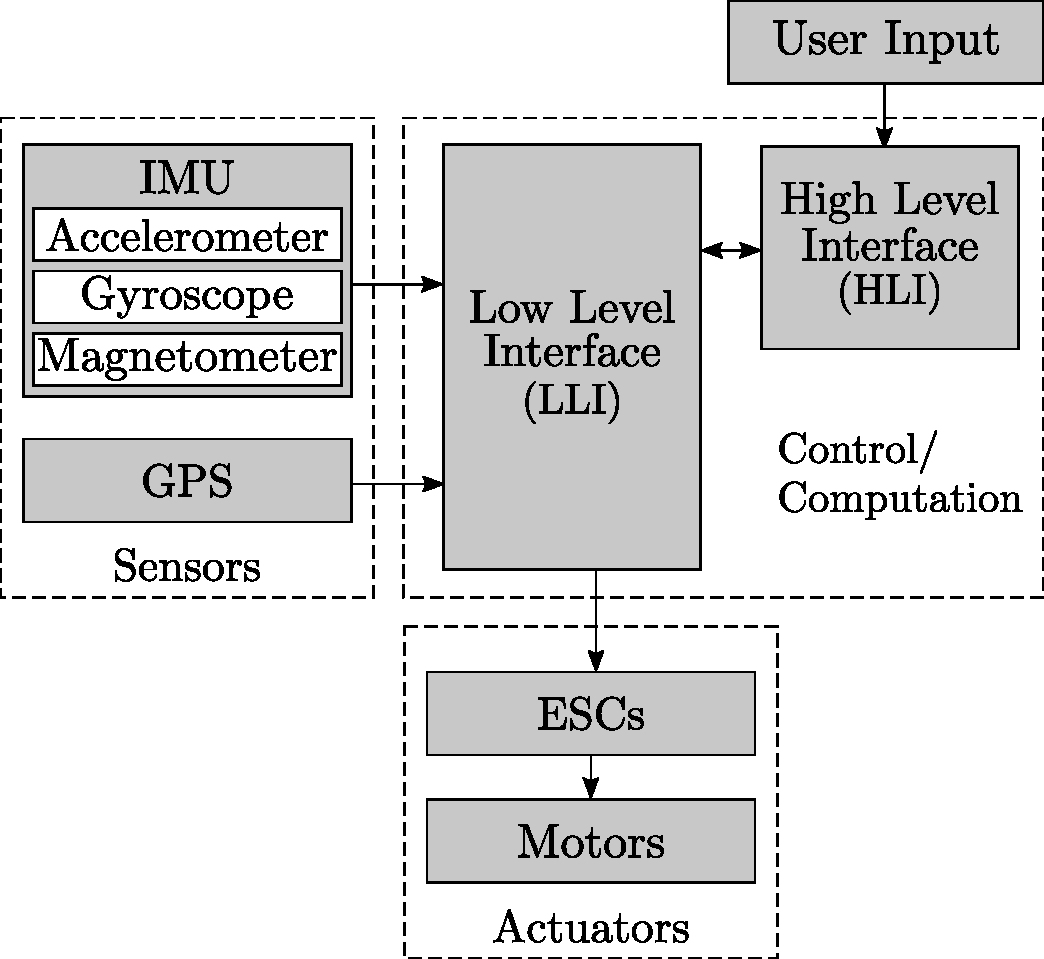
\includegraphics[width=0.6\textwidth]{figures/systemDiagram}
    \caption{}
    \label{fig:systemDiagram}
\end{figure}

Header of the chapter.


    \section{Actuation System}
The actuation system present on the vessel is constituted by the thrusters and the ESCs.

\subsection{Thrusters}
The thrusters are the main actuators present on the vessel and they provide a forward force depending on the rotational speed of the motors.

The relationship between the command and the force that they exert have been obtained through an experimental test described in \autoref{app:forceTest}. It is as follows
%
\begin{flalign}
    \mathrm{PWM} = \num{6.6044} \ F + \num{70.0168} \ \ .
    \label{eq:backwardSpeedForce}
\end{flalign}
%
If a negative force is required, they can also rotate in the opposite direction, producing a backwards force that is calculated as 
%
\begin{flalign}
    \mathrm{PWM} = \num{8.5706} \ F - \num{91.9358} \ \ .
    \label{eq:forwardSpeedForce}
\end{flalign}
%

The thrusters are actuated with brushless motors INLINE 750 \num{14.8} V from Graupner. They have two poles with a velocity constant of 1035 rpm$\cdot$kV$^{-1}$ and can operate within \num{7.4} and \num{22.2} V, being the nominal voltage \num{14.8} V. \cite{motors}

\begin{figure}[H]
    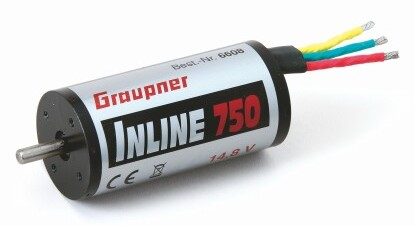
\includegraphics[width=0.4\textwidth]{figures/motor}
    \caption{INLINE 750 \num{14.8} V motor used to produce the thrust in the surface vessel \cite{motors}.}
    \label{fig:motors}
\end{figure}

\subsection{Electronic Speed Controllers}
In order to have the motors turning to the desired rotational speed, electronic speed controllers (ESCs) +70 G\num{3,5} from Graupner are used. The supply voltage ranges from 6 to 25 V and they can handle up to 70 A in continuous current. The reference PWM that comes from the microcontroller translates into a 32kHz PWM signal to the motors. \cite{ESC}

\begin{figure}[H]
    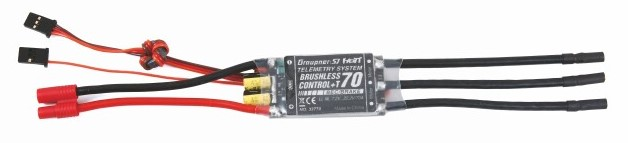
\includegraphics[width=0.8\textwidth]{figures/ESC}
    \caption{Speed controllers +70 G\num{3,5} used to control the  thrusters in the surface vessel \cite{ESC}.}
    \label{fig:ESC}
\end{figure}

%\subsection{Side Thrusters}
%The side thrusters move the vessel sideways but their influence in its motion is limited to low speed maneuvers and they are intended for fine positioning of the vessel. For this reason, they are not utilized in the controller design of the vessel.

    \section{Sensors}\label{sec:sensors}

The control system designed in the vessel requires the presence of sensor data that provide information about the vessel's motion. These are an Inertial Measurement Unit (IMU) and a Global Positioning System (GPS) module.

\subsection{IMU}

The Inertial Measurement Unit installed in the vessel is formed by a triaxial gyroscope with digital range scaling between ±75°/sec, ±150°/sec or ±300°/sec, a triaxial accelerometer with a range of ±18 g and a triaxial magnetometer with a range of ±\num{2.5} gauss. It also contains SPI-compatible serial interface to be able to obtain the data. \cite{IMUDatasheet}
%
\begin{figure}[H]
	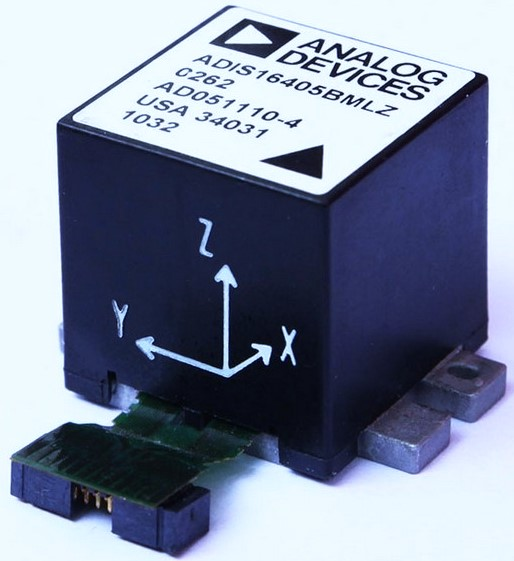
\includegraphics[width=0.3\textwidth]{figures/IMU}
	\caption{ADIS16405BMLZ IMU module mounted in the vessel \cite{IMUFigure}}
	\label{fig:IMU}
\end{figure}
%
The data provided by the IMU is used to estimate both the position and the attitude of the vessel and is extracted in the Low Level Interface through SPI serial communication.

%Triaxial, digital gyroscope with digital range scaling
%±75°/sec, ±150°/sec, ±300°/sec settings
%Tight orthogonal alignment, 0.05°
%Triaxial, digital accelerometer, ±18 g
%Triaxial, digital magnetometer, ±2.5 gauss
%SPI-compatible serial interface
%Embedded temperature sensor
%Single-supply operation: 4.75 V to 5.25 V

\subsection{GPS}
The vessel has a UP-501 GPS Receiver installed. It operates with a update frequency up to 10 Hz and its trasmits the received position data through a serial communication to the Low Level Interface. \cite{GPS}
%
\begin{figure}[H]
	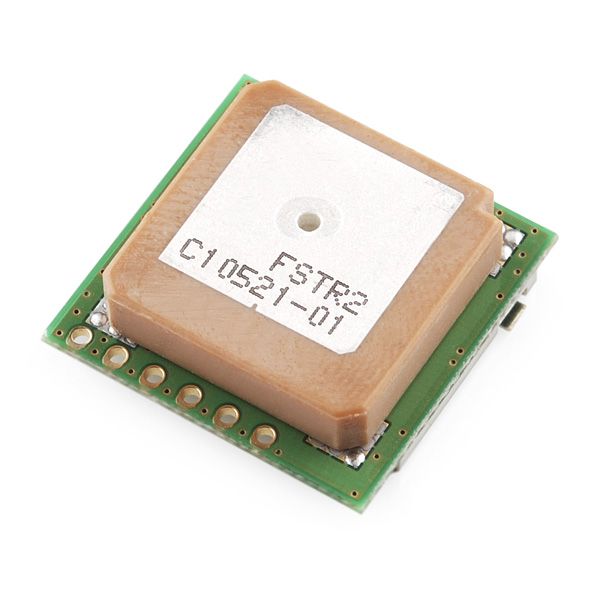
\includegraphics[width=0.3\textwidth]{figures/GPS}
	\caption{UP-501 GPS receiver mounted in the vessel \cite{GPS}.}
	\label{fig:GPS}
\end{figure}
%
As the UP-501 is a standard GPS receiver, its precision is in the range of meters \fxnote{How to prove this?? Maybe make a test.}. This makes it cumbersome to control the position of the vessel using only GPS data, and thus, the GPS and the IMU data is combined to obtained the position of the vessel.

\section{Real Time Kinematic (RTK) GPS}
\fxnote{sources incoming (:}
In addition to the UP-501 module, an Emlid Reach RTK GPS is installed. 
An RTK GPS system consists of two parts, a base station, and a rover.
The base station is set up at a stationary location with a known, precise GPS position.
The rover GPS, mounted on the ASV, measures its location, based on GPS satellites and measurements from the base station.

The base station gets its current position same as the rover using approximately the same satellites. Since the true position of the base is known, so is the error of each measurement. This is then sent as correction data to the rover, where the error is compensated for.

An RTK GPS is able to archive a higher precision than an ordinary GPS by receiving correction data from a base station.
%The correction data is used by the rover to estimate signal disturbances, caused be the signals entering the atmosphere. 
This enables it to increase the precision of the GPS measurements, from 2-5m down to a theoretical precision of a few centimeters.
This data is formatted as an RTCM3 message, which is a protocol designed for this purpose.
\begin{figure}[H]
	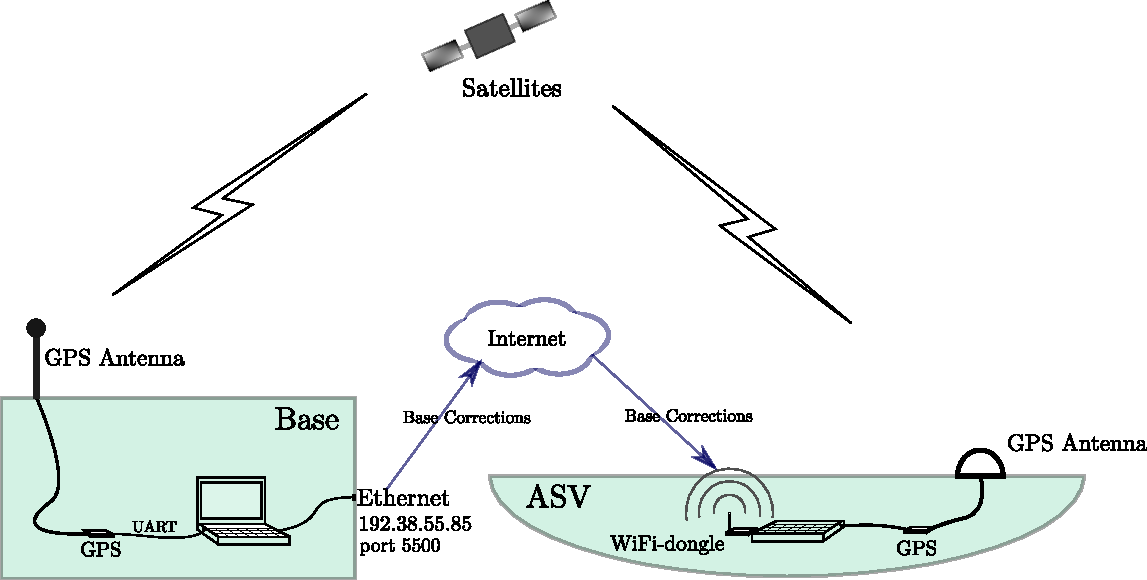
\includegraphics[width=0.6\textwidth]{figures/comunicationSetup.pdf}
	\caption{Overall set up of GPS}
	\label{fig:rtk_GPS}
\end{figure}
\autoref{fig:rtk_GPS} shows how the RTK GPS system is set up. 
The computer runs a Python script which forwards the message to a TCP socket, making it accessible through the Internet. 
The HLI on the vessel connects to this socket and feeds the data to the Rover located on the boat.
For a more detailed description of the setup see \autoref{app:rtk_gps}

    \section{Processing Units}\label{sec:ControlComputation}
The processing units take the sensor data and computes the required actuation output according to the desired motion for the vessel. It is structured in two entities that run in different devices. These entities are the Low Level Interface (LLI) and the High Level Interface (HLI).

\subsection{Low Level Interface} 
The LLI implemented on the vessel runs on a Arduino Mega Development board with and Atmel microcontroller ATMEGA 2560. It is in charge of extracting the sensor data from the IMU and send it to the HLI that runs on the computer. This includes managing the serial communication from the sensors to the Arduino Board and from the Arduino Board to the HLI. 

The LLI also handles the actuators as it receives the command for the thrusters from the HLI and calculates the appropriate PWM so the ESCs make the motors turn at the desired speed.

\subsection{High Level Interface}

The HLI takes care of the control, sensor fusion and trajectory planning algorithms. This includes communicating with the LLI to get sensor data and send commands to the thrusters. 

The HLI is implemented in a ASUS Eee Computer \cite{asus} that runs with Ubuntu 14.04 \cite{ubuntu}. In order to implement the aforementioned algorithms, the Robotic Operating System (ROS) is used. ROS allows programming the different tasks without considering the transmission of data between threads, as this is managed by ROS using its structure of nodes an topics. Besides communication between tasks, it also includes multiple tools and capabilities useful for trajectory planning, computer vision\fxnote{we should probably not mention the vision here?} and others \cite{ROS}.
    
    %---------- Chapter 3 ---------------------------------------- Modeling
    \chapter{System Model} \label{chap:model}
The model of the surface vessel is based in the methods presented in \cite{TFossen}, where the main dynamic effects regarding the behavior of the vessel are taken into account and  described in order to generate a model that serves as a basis for control design and simulations.


    \section{Background}
The model of the surface vessel is based in the hydrodynamic modeling presented in \cite{TFossen}, where the principal effects that need to be taken into account are described.

In this section, the different contributions are summarized and related to the vessel at hand.

\subsection{Reference Frames}
To describe the orientation and position of the surface vessel two coordinate frames are used, the body frame and an inertial frame. For operations in a local area, with longitude and latitude approximately constants (flat navigation) a NED system (North-East-Down) can be assumed as an inertial frame where Newton's physics will apply \cite[p. 17]{TFossen}.

To distinguish between the two frames, the body frame is denoted by a subindex "$_\mathrm{b}$", and the inertial frame with subindex "$_\mathrm{n}$". In \autoref{fig:refFrame}, a diagram of the surface vessel with the notation used can be seen.

\begin{figure}[H]
    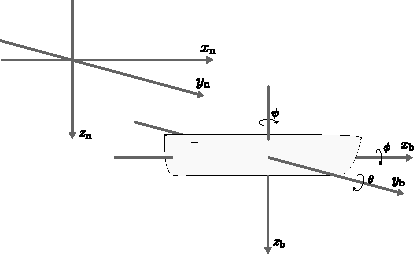
\includegraphics[width=0.6\textwidth]{figures/boat3D}
    \caption{$x_\mathrm{b}$, $y_\mathrm{b}$ and $z_\mathrm{b}$ refer to the position with respect to the body coordinate frame, while $x_\mathrm{n}$, $y_\mathrm{n}$ and $z_\mathrm{n}$ describe it with respect to the inertial frame. $\phi$, $\theta$ and $\psi$ refer to the rotation around $x_\mathrm{b}$, $y_\mathrm{b}$ and $z_\mathrm{b}$, respectively.}
    \label{fig:refFrame}
\end{figure}


The transformation from the body frame to the inertial can be done through a rotation matrix, \eqref{eq:RotMatrix}, which describes a total rotation in terms of three consecutive rotations.

In this case the rotation matrix is composed with a 1-2-3 convention, that is, first a rotation around $x_{\mathrm{b}}$, then around $y_{\mathrm{b}}$ and finally around $z_{\mathrm{b}}$ \cite[p. 22]{TFossen}.

\begin{minipage}{0.32\linewidth}
    \begin{flalign}
    \vec{R}_\mathrm{X} &=
    \begin{bmatrix}
    1 & 0      & 0       \\ 
    0 & c\phi  & -s\phi  \\ 
    0 & s\phi  & c\phi   \nonumber  
    \end{bmatrix} 	\label{eq:RotMatrix1}
    \end{flalign}
\end{minipage}\hfill
\begin{minipage}{0.32\linewidth}
    \begin{flalign}
    \vec{R}_\mathrm{Y} &=
    \begin{bmatrix}
    c\theta  & 0  & s\theta  \\ 
    0          & 1  & 0      \\ 
    -s\theta & 0  & c\theta  \nonumber 
    \end{bmatrix} 	\label{eq:RotMatrix2}
    \end{flalign}
\end{minipage}\hfill
\begin{minipage}{0.32\linewidth}
    \begin{flalign}
    \vec{R}_\mathrm{Z} &=
    \begin{bmatrix}
    c\psi & -s\psi  & 0  \\ 
    s\psi & c\psi   & 0  \\ 
    0       & 0         & 1  \nonumber 
    \end{bmatrix} 	\label{eq:RotMatrix3}
    \end{flalign}
\end{minipage}\hfill
\small
\begin{flalign}
\vec{R}^\mathrm{n}_\mathrm{b} = \vec{R}_Z \vec{R}_Y \vec{R}_X =
\begin{bmatrix}
c\theta c\psi  & s\phi s\theta c\psi -c\phi s\psi  & c\phi s\theta c\psi + s\phi s\psi  \\ 
c\theta s\psi  & s\phi s\theta s\psi + c\phi c\psi & c\phi s\theta s\psi - s\phi c\psi  \\ 
-s\theta         & s\phi c\theta                           & c\phi c\theta
\end{bmatrix} 	\label{eq:RotMatrix}
\end{flalign}
\normalsize
%
\begin{where}
    \va{\vec{R}_\mathrm{X}}{is the matrix describing a rotation around the $x_\mathrm{b}$ axis}{}
    \va{\vec{R}_\mathrm{Y}}{is the matrix describing a rotation around the $y_\mathrm{b}$ axis}{}
    \va{\vec{R}_\mathrm{Z}}{is the matrix describing a rotation around the $z_\mathrm{b}$ axis}{}
    \va{\vec{R}^\mathrm{n}_\mathrm{b}}{is the total rotation matrix}{}
\end{where}

Note that due to the size of the matrix sine and cosine are denoted $s$ and $c$ respectively.

To describe a vector in the inertial frame given its description in the body frame, a matrix-vector multiplication can be done as follows:
%
\begin{flalign}
v_{\mathrm{n}}=\vec{R}^\mathrm{n}_\mathrm{b}v_\mathrm{b} 
\end{flalign}
\begin{where}
    \va{v_{\mathrm{n}}}{is a column vector that contains the description with respect to the inertial frame}{}
    \va{v_{\mathrm{b}}}{is a column vector that contains the description with respect to the body frame}{}
\end{where}

If the inverse computation is needed, it can be done following the same procedure using $\vec{R}^\mathrm{n\ T}_\mathrm{b}$ as the rotation matrix.    

\subsection{Rigid Body Dynamics}

The first step to model the motion of the surface vessel is to look at its rigid body dynamics. They are described assuming that the center of gravity of the boat coincides with the origin of the body coordinate frame.

The translational movement can be analyzed using Newton's second law, where the acceleration of the vessel is related to the applied forces.
%
\begin{flalign}
\sum F=m \ddot{x}
\end{flalign}
%
In the case of the rotational movement, the motion is describe using the Newton's second law applied to rotational movement, where the torques applied to the system influence the angular acceleration in each axis.
%
\begin{flalign}
\sum \tau=I \ddot{\theta}
\end{flalign}
%
%The movement can be influence by the Coriolis effect, due to the fact that the body coordinate frame rotates with respect to the inertial frame. This effect, however, can be neglected in the case of a small vehicle that moves slow such as the vessel at hand \finite{find source}.
This movement is subject to the Coriolis effect, which appear if the vessel is not rotating around the axis with least- or highest- inertial axis.
The influence of this force is small if the vessel rotates at low speeds, hence it have been neglected in the model.

\subsection{Hydrostatics}

The hydrostatics describe what forces and torques are applied on the surface vessel by the volume of fluid displaced when floating on water. The force induced upon the vessel is called buoyancy force and it is applied to the center of buoyancy.  

The buoyancy force acts in the negative $z_\mathrm{n}$ direction as seen in
%
\begin{flalign}
B = \rho g (V + \Delta V(z))
\end{flalign}
\begin{where}
    \va{\rho}{is the density of the fluid in which the vessel floats}{kg m^{-3}}
    \va{g}{is the gravitational acceleration}{m s^{-2}}
    \va{V}{is the volume of fluid displaced by the surface vessel}{m^3}
    \va{\Delta V}{is the change in volume of fluid displaced by the surface vessel}{m^3}
    \va{B}{is the buoyancy force}{N}
\end{where}

When the vessel floats, the gravity force cancels out $ \rho g V $ of the buoyancy force, making the contribution of the latest along $x_\mathrm{b}$, $y_\mathrm{b}$ and $z_\mathrm{b}$ directions dependent only on the variation with respect to the equilibrium flotation point.
This result is seen in 
%
\begin{flalign}
F_{z_\mathrm{n}} = mg - \rho g V -\rho g  \Delta V(z) = -\rho g  \Delta V(z) 
\end{flalign}
\begin{where}
    \va{F_{z_\mathrm{n}}}{is the summation of forces along the $z_\mathrm{n}$ direction}{N}
\end{where}

The change in volume can be expressed as in \autoref{eq:deltaV}. The water plane of the vessel is not considered to vary significantly with change in vertical position, thus the approximation seen in the equation is applied.
%
\begin{flalign}
\Delta V(z) = \int_{0}^{z_\mathrm{N}}A_\mathrm{wp}(\zeta)d\zeta \approx A_\mathrm{wp}z_\mathrm{n}
\label{eq:deltaV}
\end{flalign}
\begin{where}
    \va{A_\mathrm{wp}}{is the water plane area of the vessel}{m^2}
\end{where}

The contribution along the body frame directions is calculated as a function of the $\phi$ and $\theta$ angles in  
%
\begin{flalign}
F_{x_\mathrm{b}} &= -\rho g A_\mathrm{wp}z_\mathrm{n} (-\sin \theta)  \\
F_{y_\mathrm{b}} &= -\rho g A_\mathrm{wp}z_\mathrm{n} (\cos \theta \sin \phi)  \\
F_{z_\mathrm{b}} &= -\rho g A_\mathrm{wp}z_\mathrm{n} (\cos \theta \cos \phi) 
\label{eq:forcez}
\end{flalign}

If the variations of $\phi$ and $\theta$ are small, the contribution of the buoyancy force in the $x_\mathrm{b}$ and $y_\mathrm{b}$ directions can be neglected and not included in the final model of the vessel. \cite[pp. 62-67]{TFossen}

The buoyancy force also contributes with some torques around the different axis in the body coordinate frame. This occurs as the center of buoyancy in general is not aligned with the center of gravity, generating some restoring torques on the vessel. These torques are dependent on the gravity and the buoyancy force. As the contribution of the term $\rho g \Delta V$ is small compared to that of $\rho g V$, only the latter is considered in the model.  \cite[pp. 62-67]{TFossen}
%
\begin{flalign}
T_{\phi} &= -\rho g V \overline{GM}_{\mathrm{T}} \sin \phi (\cos \theta \cos \phi)   
\label{eq:torqphi} \\
T_{\theta} &= -\rho g V \overline{GM}_{\mathrm{L}} \sin \theta (\cos \theta \cos \phi) 
\label{eq:torqtheta}
\end{flalign}
\begin{where}
    \va{T_{\phi}}{is the restoring torque due to the buoyancy force in the $\phi$ direction}{Nm}
    \va{T_{\theta}}{is the restoring torque due to the buoyancy force in the $\theta$ direction}{Nm}
    \va{\overline{GM}_\mathrm{T}}{is the transverse metacentric height}{m}
    \va{\overline{GM}_\mathrm{L}}{is the longitudinal metacentric height}{m}
\end{where}

The metacentric heights are the distances between the center of gravity and the metacenter of the vessel. The metacenter position is related with the position of the center of gravity and that of the center of buoyancy. \cite[pp. 65-67]{TFossen}
%equations in the book page 78

\subsection{Hydrodynamics}
The hydrodynamic forces induced in the surface vessel are mainly caused by two terms. The added mass and the viscous damping.

The added mass induces forces that originate from the vessel imposing some energy in the surrounding fluid when it moves through it. The force generated is dependent on the acceleration of the vessel. \fxnote{what to do here??}

The viscous damping is a combination of several factors, namely, skin friction, wave drift damping and vortex shedding \cite[p. 122]{TFossen}. This type of damping appears in the equations as coefficients that multiply, with negative sign, the different translational and angular velocities that define the movement of the vessel. For each degree of freedom it is expressed as
%
\begin{flalign}
D_{\dot{x}_\mathrm{b}} &= - d_{\dot{x}_\mathrm{b}}  \dot{x}_\mathrm{b} \\
D_{\dot{y}_\mathrm{b}} &= - d_{\dot{y}_\mathrm{b}}  \dot{y}_\mathrm{b} \\
D_{\dot{z}_\mathrm{b}} &= - d_{\dot{z}_\mathrm{b}}  \dot{z}_\mathrm{b} \\
D_{\dot{\phi}} &= - d_{\dot{\phi}}                  \dot{\phi} \\
D_{\dot{\theta}} &= - d_{\dot{\theta}}              \dot{\theta} \\
D_{\dot{\psi}} &= - d_{\dot{\psi}}                  \dot{\psi}  \\
\end{flalign}
\begin{where}
    \va{D_{i}}{is the damping force or torque due to viscous damping.}{}
    \va{d_{i}}{is the viscous damping coefficient.}{}
\end{where}

This equation consider that the viscous friction is linear, this assumption can be done for vessel speeds lower than 2 m/s \cite[p. 138]{TFossen}. 

    \section{Model Equations}   
The final model equations are presented in this section, and are described relative to the body frame, meaning that all movement is relative to the vessel.
\autoref{fig:boat3DForces} and \ref{fig:boat2D} show a diagram of the vessel.
\begin{figure}[H]
    \captionbox
    {
        Diagram of the vessel, where the forces applied by the motors are shown.
        \label{fig:boat3DForces}
    }
    {
        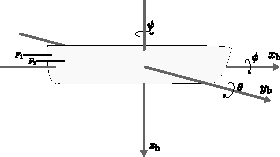
\includegraphics[width=.54\textwidth]{figures/boat3DForces}
    }
    \hspace{5pt}
    \captionbox
    {
        Top view of the vessel, where the distances needed for the model equations are also presented.
        \label{fig:boat2D}
    }
    {
        \hspace{1.1cm} 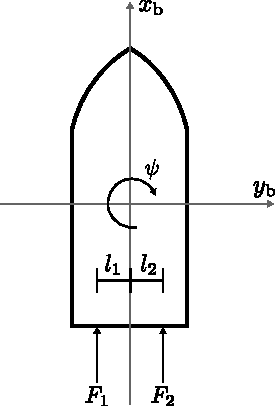
\includegraphics[width=.24\textwidth]{boat2D} \hspace{1.1cm}
    }
\end{figure}

The translational movement of the vessel is described by \autoref{eq:x_pos_model}, \ref{eq:y_pos_model} and \ref{eq:z_pos_model}.
The model includes the forces applied by the motors and the damping, that create an acceleration in the vessel as
%
\begin{flalign}
	m \ddot{x}_\mathrm{b} &=  F_\mathrm{1} + F_\mathrm{2}  - d_{\dot{x}_\mathrm{b}} \dot{x}_\mathrm{b} + F_{x_\mathrm{b}}
    \label{eq:x_pos_model} \ ,\\
    m \ddot{y}_\mathrm{b} &=  -d_{\dot{y}_\mathrm{b}} \dot{y_\mathrm{b}} + F_{y_\mathrm{b}}
    \label{eq:y_pos_model} \ ,\\
    m \ddot{z}_\mathrm{b} &=  -d_{\dot{z}_\mathrm{b}}\dot{z_\mathrm{b}} + F_{z_\mathrm{b}} \ . \label{eq:z_pos_model}
\end{flalign}
%
\begin{where}
	\va{m}{is the mass of the vessel}{kg}
    \va{\ddot{x}_\mathrm{b}}{is the acceleration in the $x_\mathrm{b}$ direction}{m \cdot s^{-2}}
    \va{\ddot{y}_\mathrm{b}}{is the acceleration in the $y_\mathrm{b}$ direction}{m \cdot s^{-2}}
    \va{\ddot{z}_\mathrm{b}}{is the acceleration in the $z_\mathrm{b}$ direction}{m \cdot s^{-2}}
    \va{\dot{x}_\mathrm{b}}{is the velocity in the $x_\mathrm{b}$ direction}{m \cdot s^{-1}}
    \va{\dot{y}_\mathrm{b}}{is the velocity in the $y_\mathrm{b}$ direction}{m \cdot s^{-1}}
    \va{\dot{z}_\mathrm{b}}{is the velocity in the $z_\mathrm{b}$ direction}{m \cdot s^{-1}}
    \va{F_{1,2}}{are the forces applied by each motor}{N}
\end{where}

%The virtual mass components are the added mass from the displaced water in the respective direction plus the mass of the vessel. This value is different for each axis, as the difference in shape drags a different amount of water.
    
The rotational movement of the vessel is described by \autoref{eq:phi_model}, \ref{eq:theta_model} and \ref{eq:psi_model}.
%
\begin{flalign}
    I_\mathrm{x}\ddot{\phi} &= -d_{\dot{\phi}} \dot{\phi} + T_\mathrm{\phi}  \ ,
    \label{eq:phi_model} \\
    I_\mathrm{y}\ddot{\theta} &= -d_{\dot{\theta}} \dot{\theta} + T_\mathrm{\theta}  \ ,
    \label{eq:theta_model} \\
    I_\mathrm{z}\ddot{\psi} &= F_\mathrm{1}l_\mathrm{1} - F_\mathrm{2} l_\mathrm{2} - d_{\dot{\psi}} \dot{\psi} \ . \label{eq:psi_model}
\end{flalign}
%
\begin{where}
    \va{I_\mathrm{x}}{is the inertia around the $x_\mathrm{b}$ axis}{kg \cdot m^2}
    \va{I_\mathrm{y}}{is the inertia around the $y_\mathrm{b}$ axis}{kg \cdot  m^2}
    \va{I_\mathrm{z}}{is the inertia around the $z_\mathrm{b}$ axis}{kg \cdot  m^2}
    \va{\ddot{\phi}}{is the angular acceleration around the $x_\mathrm{b}$ axis}{rad\cdot s^{-2}}
    \va{\ddot{\theta}}{is the angular acceleration around the $y_\mathrm{b}$ axis}{rad \cdot s^{-2}}
    \va{\ddot{\psi}}{is the angular acceleration around the $z_\mathrm{b}$ axis}{rad \cdot s^{-2}}
    \va{\dot{\phi}}{is the angular velocity around the $x_\mathrm{b}$ axis}{rad \cdot s^{-1}}
    \va{\dot{\theta}}{is the angular velocity around the $y_\mathrm{b}$ axis}{rad \cdot s^{-1}}
    \va{\dot{\psi}}{is the angular velocity around the $z_\mathrm{b}$ axis}{rad \cdot s^{-1}}
    \va{l_1}{is the perpendicular distance from motor 1 to the center of gravity}{m}
    \va{l_2}{is the perpendicular distance from motor 2 to the center of gravity}{m}
\end{where}

Similar to the translational equations, only one axis is controllable. This is, however, not a problem in practice, since the vessel is stable by nature and it can be controlled even being an underactuated vehicle \cite[pp. 235-239]{TFossen}.

    \section{Linearization of Model Equations}\label{sec:linearizationModel}
The model equations need to be linearized to design a controller using linear techniques. This is done using the first order Taylor approximation around an equilibrium point as seen in 
%
\begin{flalign}
    f(x) &\approx f(\overline{x}) + f'(\overline{x}) (x-\overline{x})  \rightarrow\ \tilde{f}(x) \approx f'(\overline{x}) \tilde{x} \ .
    \label{taylor}
\end{flalign}

In this equation, $\overline{x}$ represents the equilibrium point and $\tilde{x}$ the change from the equilibrium point.

The equilibrium point must fulfill that all the derivatives of the states are zero, in this case the velocities and accelerations. This implies that the resulting forces and torques must be zero. 

To apply the approximation, the function must be differentiated with respect to each of the present variables, and once linearized, the function is expressed in terms of variations from the equilibrium point.
%
\begin{flalign}
    f &= f(x_1,x_2,...,x_\mathrm{n}) \nonumber \ ,\\
    \tilde{f}&=\frac{\partial f}{\partial x_1}\bigg|_{\overline{x}_1,\overline{x}_2,...,\overline{x}_n}\ \tilde{x}_1 + \frac{\partial f}{\partial x_2}\bigg|_{\overline{x}_1,\overline{x}_2,...,\overline{x}_n}\ 
    \tilde{x}_2+...+ \frac{\partial f}{\partial x_n}\bigg|_{\overline{x}_1,\overline{x}_2,...,\overline{x_n}}\ \tilde{x}_\mathrm{n} \ . \nonumber
    \label{eq:dummytaylor}
\end{flalign}
%
In the case of the vessel, the only nonlinear terms are the restoring forces and torques. They can be linearized, giving the following results
\begin{flalign}
    \tilde{F}_{x_\mathrm{b}} &= 0  \label{eq:forcexlin} \ ,\\
    \tilde{F}_{y_\mathrm{b}} &= 0  \label{eq:forceylin} \ ,\\
    \tilde{F}_{z_\mathrm{b}} &= -\rho g A_\mathrm{wp} \tilde{z}_\mathrm{n} \label{eq:forcezlin} \ , \\
 	\tilde{T}_{\phi} &= -\rho g V \overline{GM_{T}}\cdot \tilde{\phi} \label{eq:torquephilinar} \ , \\
    \tilde{T}_{\theta} &= -\rho g V \overline{GM_{L}}\cdot \tilde{\theta} \ .\label{eq:torquethetalinar}   
\end{flalign}
%
From now on, the linearized variables are represented without the symbol "$\sim$", to avoid excessive notation, even though they refer to changes with respect to the the equilibrium point.

The model equations including these linearized terms end up being
%
\begin{flalign}
 	m_\mathrm{x} \ddot{x}_\mathrm{b} &=  F_\mathrm{1} + F_\mathrm{2}  - d_{\dot{x}_\mathrm{b}} \dot{x}_\mathrm{b}
     \label{eq:x_pos_model_lin} \ , \\
    m_\mathrm{y} \ddot{y}_\mathrm{b} &=  -d_{\dot{y}_\mathrm{b}} \dot{y_\mathrm{b}}
     \label{eq:y_pos_model_lin} \ , \\
    m_\mathrm{z} \ddot{z}_\mathrm{b} &=  -d_{\dot{z}_\mathrm{b}}\dot{z_\mathrm{b}} -\rho g A_\mathrm{wp} \tilde{z}_\mathrm{n} \label{eq:z_pos_model_lin} \ ,  \\
    I_\mathrm{x}\ddot{\phi} &= -d_{\dot{\phi}} \dot{\phi} - \rho g V \overline{GM_{T}}\cdot \phi
    \label{eq:phi_model_limn} \ , \\
    I_\mathrm{y}\ddot{\theta} &= -d_{\dot{\theta}} \dot{\theta} - \rho g V \overline{GM_{L}}\cdot \theta
    \label{eq:theta_model_lin} \ , \\
    I_\mathrm{z}\ddot{\psi} &= F_\mathrm{1}l_\mathrm{1} - F_\mathrm{2} l_\mathrm{2} - d_{\dot{\psi}} \dot{\psi} \ . \label{eq:psi_model_lin}
\end{flalign}



%\begin{flalign}
%    m_\mathrm{x} \ddot{x}_\mathrm{b} &=  F_\mathrm{1} + F_\mathrm{2}  - d_\mathrm{x} \dot{x}_\mathrm{b} + m_\mathrm{y} \dot{y_\mathrm{b}} \dot{\psi} - m_\mathrm{z} \dot{z}_\mathrm{b} \dot{\theta} - F_\mathrm{x}
%    \label{eq:x_pos_model} \\
%    m_\mathrm{y} \ddot{y_\mathrm{b}} &=  -d_\mathrm{y}\dot{y_\mathrm{b}}-m_\mathrm{x}\dot{x_\mathrm{b}}\dot{\psi}+m_\mathrm{z}\dot{z_\mathrm{b}}\dot{\phi}-F_\mathrm{y}
%    \label{eq:y_pos_model} \\
%    m_\mathrm{z} \ddot{z_\mathrm{b}} &=  -d_\mathrm{z}\dot{z_\mathrm{b}}+ m_\mathrm{b}\dot{x_\mathrm{b}}\dot{\theta}-m_\mathrm{y}\dot{y_\mathrm{b}} \dot{\phi}-F_\mathrm{z} \label{eq:z_pos_model}
%\end{flalign}
%
%\begin{flalign}
%    I_\mathrm{x}\ddot{\phi} &= -d_\mathrm{\phi} \dot{\phi}-(m_\mathrm{z}-m_\mathrm{y}) \dot{z}_\mathrm{b} \dot{y}_\mathrm{b}-(I_\mathrm{z}-I_\mathrm{y}) \dot{\theta } \dot{\psi}+T_\mathrm{\phi}  
%    \label{eq:x_inert_model} \\
%    I_\mathrm{y}\ddot{\theta} &= -d_\mathrm{\theta} \dot{\theta}-(m_\mathrm{z}-m_\mathrm{x}) \dot{x}_\mathrm{b} \dot{y}_\mathrm{b}-(I_\mathrm{x}-I_\mathrm{z}) \dot{\phi} \dot{\psi}+T_\mathrm{\theta}  
%    \label{eq:y_inert_model} \\
%    I_\mathrm{z}\ddot{\psi} &= -d_\mathrm{\psi} \dot{\psi}-(m_\mathrm{y}-m_\mathrm{x}) \dot{x}_\mathrm{b}\dot{y}_\mathrm{b}-(I_\mathrm{z}-I_\mathrm{y})\dot{\psi}\dot{\theta}+F_\mathrm{1}l_\mathrm{1}+F_\mathrm{2}l_\mathrm{2}+T_\mathrm{\psi} \label{eq:z_inert_model}
%\end{flalign}

    
    %---------- Chapter 4 ---------------------------------------- Controller Design
    \chapter{Controller Design}

Header of control chapter

\begin{figure}[H]
    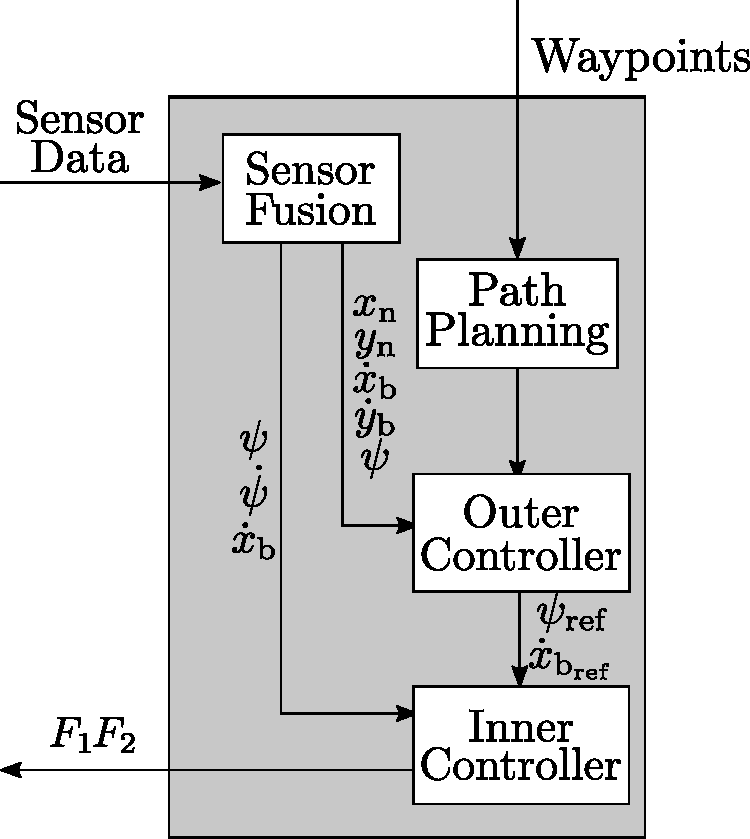
\includegraphics[width=0.8\textwidth]{figures/controllerDiagram}
    \caption{}
    \label{fig:controllerDiagram}
\end{figure}
    \section{State Space Model}\label{chap:control}

The linearized model derived in \autoref{sec:linearizationModel}, consisting of \autoref{eq:x_pos_model_lin} to \ref{eq:psi_model_lin} needs to be represented in state space form in order to design a state space controller. In order to do that, the 3 degree of freedom model used for the control of the vessel is represented as
\begin{flalign}
  \vec{\dot{x}}(t) &= \vec{A} \vec{x}(t) + \vec{B} \vec{u}(t)
  \label{xDotLinear} \\
  \vec{y}(t) &= \vec{C} \vec{x}(t) + \vec{D} \vec{u}(t)
  \label{yLinear} 
\end{flalign}
\begin{where}
  \va{\vec{x}}{is the state vector}{}
  \va{\vec{u}}{is the input vector}{}
  \va{\vec{y}}{is the output vector}{}
  \va{\vec{A}}{is the state matrix}{}
  \va{\vec{B}}{is the input matrix}{}
  \va{\vec{C}}{is the output matrix}{}
  \va{\vec{D}}{is the feed-forward matrix}{}
\end{where}
%
The state vector is constituted by the angle and velocity in yaw as well as the velocity in x in the body frame. The outputs of the system are yaw angle and velocity in x in the body frame. The input to the system is composed of the two forces applied in the body frame.
%It is important to notice that the position of the vessel in the body reference frame represents the  integration of the velocity along the body frame directions.
%This can also be seen as the position of the vessel with respect to a frame whose origin coincides with that of the NED frame and whose orientation coincides with that of the body frame \cite[p. 173]{TFossen}. 

\begin{minipage}{0.32\linewidth}
  \begin{flalign}
    \vec{x(t)} = 
    \begin{bmatrix}
      \psi\\
      \dot{\psi}\\
      x_{B} \\
    \end{bmatrix} \nonumber
    \label{xVector}
  \end{flalign}  
\end{minipage}\hfill
%\hspace{0.03\linewidth}
\begin{minipage}{0.32\linewidth}
  \begin{flalign}
    \vec{y(t)} = 
    \begin{bmatrix}
      \phi \\
      x_{B} \\
    \end{bmatrix} \nonumber
    \label{yVector}
  \end{flalign}
\end{minipage}\hfill
%\hspace{0.03\linewidth}
\begin{minipage}{0.32\linewidth}
  \begin{flalign}
    \vec{u(t)}= 
    \begin{bmatrix}
      F_1 \\
      F_2 
    \end{bmatrix}
    \label{uVector}
  \end{flalign} \nonumber
\end{minipage}\hfill

The resulting $\vec{A}$, $\vec{B}$, $\vec{C}$ and $\vec{D}$ matrices are
\begin{flalign}
  \vec{A} &=
  \begin{bmatrix}
    \ 0 & 1                   & 0                \ \ \ \\ 
    \ 0 & -\frac{d_\psi}{I_z} & 0                \ \ \ \\ 
    \ 0 & 0                   & -\frac{d_x}{m_x} \ \ \     
  \end{bmatrix}\rule{30px}{0px}
    \vec{B} = 
  \begin{bmatrix}
    \ 0               & 0                \ \ \ \\
    \ \frac{l_1}{I_z} & -\frac{l_2}{I_z} \ \ \ \\   
    \ \frac{1}{m_x}   & \frac{1}{m_x}    \ \ \
  \end{bmatrix}\rule{30px}{0px}
  \vec{C} =   
  \begin{bmatrix}
    \ 1 & 0 & 0  \ \ \ \\ 
    \ 0 & 0 & 1  \ \ \    
  \end{bmatrix}
   \label{eqStateSpaceABC}
\end{flalign}
and the $\vec{D}$ matrix is zero.

    \section{Linear Quadratic Regulator} \label{sec:lqr}
The first design approach for the inner controller is a state feedback. The compensator gain is obtained using a Linear Quadratic Regulator (LQR). First, a state space model of the system is created based on the equations derived in \autoref{chap:model}. Then, a cost function based on the state errors and the input usage is minimized in order to calculate the controller gains. 

\subsection{State Space Model}
The linearized model derived in \autoref{sec:linearizationModel}, consisting of \autoref{eq:x_pos_model_lin} to \ref{eq:psi_model_lin}, needs to be represented in state space form in order to design a state space controller. In order to do that, the 3 degree of freedom model used for the control of the vessel is represented as
\begin{flalign}
    \vec{\dot{x}}(t) &= \vec{A} \vec{x}(t) + \vec{B} \vec{u}(t)
    \label{xDotLinear} \\
    \vec{y}(t) &= \vec{C} \vec{x}(t) + \vec{D} \vec{u}(t)
    \label{yLinear} 
\end{flalign}
\begin{where}
    \va{\vec{x}}{is the state vector}{}
    \va{\vec{u}}{is the input vector}{}
    \va{\vec{y}}{is the output vector}{}
    \va{\vec{A}}{is the state matrix}{}
    \va{\vec{B}}{is the input matrix}{}
    \va{\vec{C}}{is the output matrix}{}
    \va{\vec{D}}{is the feed-forward matrix}{}
\end{where}

The state vector is constituted by the angle and velocity in yaw as well as the velocity in x in the body frame. The outputs of the system are yaw angle and velocity in x in the body frame. The input to the system is composed of the two forces applied in the body frame.
%It is important to notice that the position of the vessel in the body reference frame represents the  integration of the velocity along the body frame directions.
%This can also be seen as the position of the vessel with respect to a frame whose origin coincides with that of the NED frame and whose orientation coincides with that of the body frame \cite[p. 173]{TFossen}. 

\begin{minipage}{0.32\linewidth}
    \begin{flalign}
        \vec{x(t)} = 
        \begin{bmatrix}
            \psi\\
            \dot{\psi}\\
            \dot{x}_{b} \\
        \end{bmatrix} \nonumber
        \label{xVector}
    \end{flalign}  
\end{minipage}\hfill
%\hspace{0.03\linewidth}
\begin{minipage}{0.32\linewidth}
    \begin{flalign}
        \vec{y(t)} = 
        \begin{bmatrix}
            \phi \\
            \dot{x}_{b} \\
        \end{bmatrix} \nonumber
        \label{yVector}
    \end{flalign}
\end{minipage}\hfill
%\hspace{0.03\linewidth}
\begin{minipage}{0.32\linewidth}
    \begin{flalign}
        \vec{u(t)}= 
        \begin{bmatrix}
            F_1 \\
            F_2 
        \end{bmatrix}
        \label{uVector}
    \end{flalign} \nonumber
\end{minipage}\hfill

The resulting $\vec{A}$, $\vec{B}$, $\vec{C}$ and $\vec{D}$ matrices are
\begin{flalign}
    \vec{A} &=
    \begin{bmatrix}
        \ 0 & 1                   & 0                \ \ \ \\ 
        \ 0 & -\frac{d_\psi}{I_z} & 0                \ \ \ \\ 
        \ 0 & 0                   & -\frac{d_x}{m_x} \ \ \     
    \end{bmatrix}\rule{30px}{0px}
    \vec{B} = 
    \begin{bmatrix}
        \ 0               & 0                \ \ \ \\
        \ \frac{l_1}{I_z} & -\frac{l_2}{I_z} \ \ \ \\   
        \ \frac{1}{m_x}   & \frac{1}{m_x}    \ \ \
    \end{bmatrix}\rule{30px}{0px}
    \vec{C} =   
    \begin{bmatrix}
        \ 1 & 0 & 0  \ \ \ \\ 
        \ 0 & 0 & 1  \ \ \    
    \end{bmatrix}
    \label{eqStateSpaceABC}
\end{flalign}
and the $\vec{D}$ matrix is zero.

\subsection{Controller Design}
As the controller eventually must be implemented the design is carried out in the discrete domain. To do so, it is necessary to discretize the system. A discrete state space model can be expressed as,
%
\begin{flalign}
  \vec{x}(k+1) &= \vec{A_z} \vec{x}(k) + \vec{B_z} \vec{u}(k)
  \label{xDotLinearDiscrete} \\
  \vec{y}(k)   &= \vec{C_z} \vec{x}(k) + \vec{D_z} \vec{u}(k) \ \ ,
  \label{yLinearDiscrete} 
\end{flalign}
%
where the z subindexes indicate the matrices being in the discrete domain and k is the sample index. The model is discretized using zero order hold. In \autoref{fig:discreteSSBlock} the discrete system is shown in a block diagram. The feed forward matrix is excluded as it is not present in this system.
%
\begin{figure}[H]
  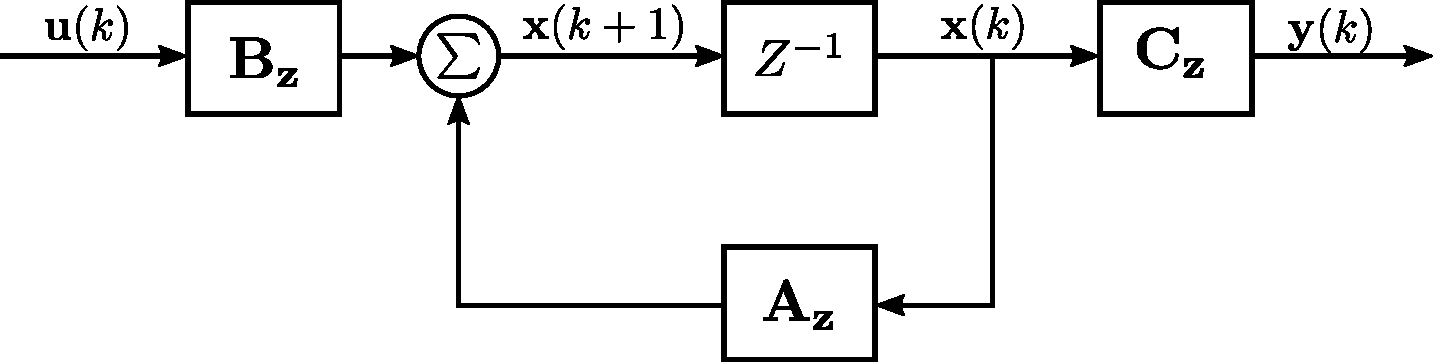
\includegraphics[width=0.6\textwidth]{figures/discreteSystemBlockDiagram}
  \caption{Block diagram of the discrete system without feed forward.}
  \label{fig:discreteSSBlock}
\end{figure}
%
In order to track a reference and handle input disturbances, it is chosen to also include an integral controller in the design. The final control structure is seen in \autoref{fig:blockConrolDesignLQR}.
%
\begin{figure}[H]
  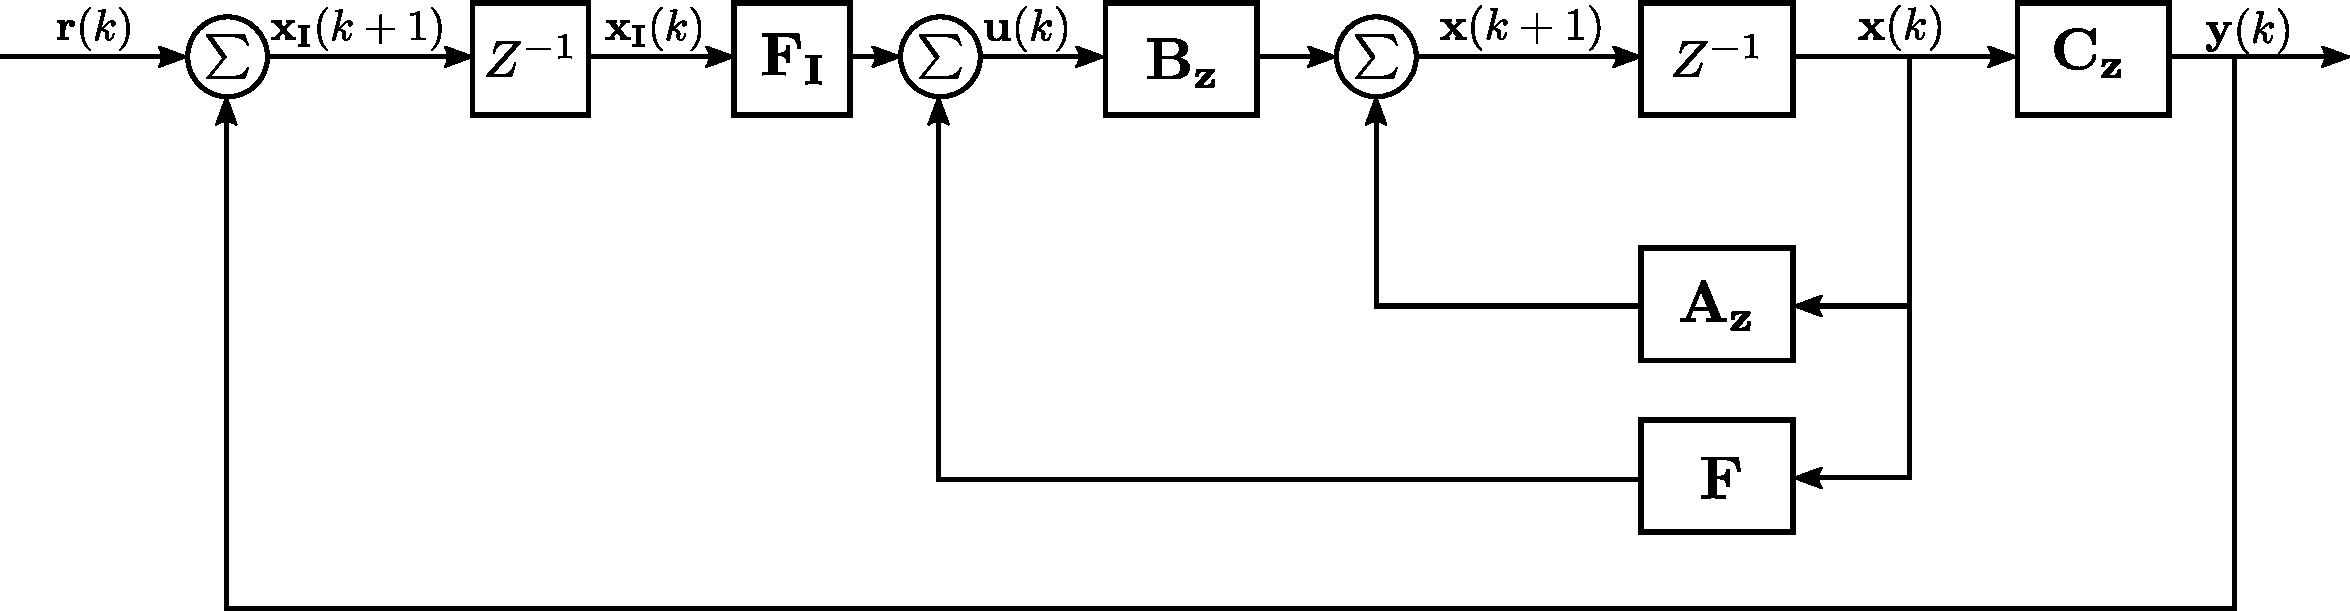
\includegraphics[width=0.9\textwidth]{figures/integralControlBlockDiagram}
  \caption{Block diagram of the control structure in the discrete domain.}
  \label{fig:blockConrolDesignLQR}
\end{figure}
%
To design this feedback system, it is convenient to express it on the following form:
\begin{flalign}
  \vec{x_e}(k+1) &= \vec{A_e} \vec{x}(k) + \vec{B_e} \vec{u}(k) + \vec{r}(k)
  \label{eq:xDotLinearDiscrete} \\
  \vec{y}(k)     &= \vec{C_e} \vec{x}(k)  \ \ .
  \label{eq:yLinearDiscrete} 
\end{flalign}
%
To describe the control design in this form, the $\vec{A_e}$, $\vec{B_e}$ and $\vec{C_e}$ matrices must be constructed. From \autoref{fig:blockConrolDesignLQR}, the discrete state space model for the integral is derived and shown in \autoref{eq:xIDiscrete}.
%
\begin{flalign}
  \vec{x_I}(k+1) &= \vec{x_I}(k) + \vec{y}(k) + \vec{r}(k) \label{eq:xIDiscrete1}  \\
  \vec{x_I}(k+1) &= \vec{x_I}(k) - C_z \vec{x}(k) + \vec{r}(k)  \ \ .
  \label{eq:xIDiscrete}
\end{flalign}
%
This leads to the discrete state space model extended with the integral states expressed as
%
\begin{flalign}
  \begin{bmatrix}
    \vec{x}(k+1)  \\
    \vec{x_I}(k+1)
  \end{bmatrix}
  =
  \begin{bmatrix}
    \vec{A}_{\vec{z}_{3x3}} & \vec{O}_{_{3x2}} \\
   -\vec{C}_{\vec{z}_{2x3}} & \vec{I}_{_{2x2}} \\
  \end{bmatrix}
  \begin{bmatrix}
    \vec{x}(k)    \\
    \vec{x_I}(k)
  \end{bmatrix}
  +
  \begin{bmatrix}
    \vec{B}_{\vec{z}_{3x2}} \\
    \vec{O}_{2x2}
  \end{bmatrix}
  \vec{u}(k)
  +
  \begin{bmatrix}
    \vec{O}_{3x2} \\
    \vec{I}_{2x2}
  \end{bmatrix}
  \vec{r}(k)
  \label{eq:discreteSSWithIntegralX}
\end{flalign}  
%
\begin{flalign}
  \vec{y}(k)
  =
  \begin{bmatrix}
    \vec{C}_{\vec{z}_{2x3}} &  \vec{O}_{2x2}
  \end{bmatrix}
  \begin{bmatrix}
    \vec{x}(k)    \\
    \vec{x_I}(k)
  \end{bmatrix}  \ \ ,
  \label{eq:discreteSSWithIntegralY}
\end{flalign}  
%
which corresponds to \autoref{eq:xDotLinearDiscrete} and \ref{eq:yLinearDiscrete}.

A discrete time infinite horizon LQR is used in the design of the feedback, $\vec{F_e} = [\ \vec{F} \ \ \vec{F}_\mathrm{I} ]\ $, which works by minimizing the cost function,
%
\begin{flalign}
  J = \sum_{k=0}^\infty \vec{x}_k^\mathrm{T}\vec{Q_d}\vec{x}_k + \vec{u}_k^\mathrm{T}\vec{R_d}\vec{u}_k  \ \ .
\end{flalign}
\begin{where}
	\va{\vec{Q_d}}{is the discrete time symmetric positive semidefinite state cost matrix}{}
  \va{\vec{R_d}}{is the discrete time symmetric positive definite input cost matrix}{}
\end{where}

The $\vec{Q_d}$ matrix contains the penalties for the states, such that a higher cost is generated for more critical states, thus driving these states faster to zero. The $\vec{R_d}$ matrix contains the penalties for the inputs. This helps to ensure the inputs are not driven towards saturation.

It is necessary for all states to be stable and controllable. Otherwise the the performance index, $J$, will become infinite \cite[p. 125]{DSNaidu}.\\
The controllability is determined by
%
\begin{flalign}
  \vec{{\mathcal C}}
  = 
  \begin{bmatrix}
    \vec{B}_\mathrm{e} & \vec{A}_\mathrm{e}\vec{B}_\mathrm{e} & \vec{A}_\mathrm{e}^{2} \vec{B}_\mathrm{e} & \vec{A}^{3}_\mathrm{e} \vec{B}_\mathrm{e} & \vec{A}^{4}_\mathrm{e} \vec{B}_\mathrm{e}
  \end{bmatrix}  \ \ ,
  \label{eq:integralControllability}
\end{flalign}
%
of which the rank is 5, that is, the controllability matrix, $\vec{{\mathcal C}}$, has full rank, thus the system is controllable \cite[p. 169]{CTChen}.\\
The eigenvalues of $\vec{A}_\mathrm{e}$ are all on or within the unit-circle in the z-plane, thus, no states are unstable and the LQR design is feasible.

The design approach taken to describe the cost function, $J$, is done by defining weights on the states and inputs for the continuous time infinite horizon LQR cost function,
%
\begin{flalign}
  J_{cont} = \int_{0}^\infty \vec{x}_k^\mathrm{T}\vec{Q}\vec{x}_k + \vec{u}_k^\mathrm{T}\vec{R}\vec{u}_k \  dt\ \ .
  \label{eq:contLQRcost}
\end{flalign}
\begin{where}
  \va{\vec{Q}}{is the continuous time symmetric positive semidefinite state cost matrix}{}
  \va{\vec{R}}{is the continuous time symmetric positive definite input cost matrix}{}
\end{where}

Bryson's rule is used as an initial design method to determine sensible values for the state and input penalties of the $\vec{Q}$ and $\vec{R}$ matrices, as described in \autoref{eq:QRBryson}\\
%
\begin{flalign} 
  Q_{ii} &= \frac{1}{x_{i_\mathrm{max}}\text{}^2} \rule{30px}{0px} R_{ii} = \frac{1}{u_{i_\mathrm{max}} \text{}^2}
  \label{eq:QRBryson}
\end{flalign}
\begin{where}
  \va{x_{i_\mathrm{max}}}{are the maximum acceptable state values}{}
  \va{u_{i_\mathrm{max}}}{are the maximum acceptable input values}{}
\end{where}

The requirements stated in \autoref{sec:requirements} must be taken into account when determining the values of $x_{i_\mathrm{max}}$ and $u_{i_\mathrm{max}}$. As the USV needs a high accuracy for bathymetric measurements, the weights of $\vec{Q}$ are set higher than $\vec{R}$ to ensure priority is focused on driving the states down to zero. The individual integral states are penalized higher than the system states to set further importance on driving the integral states to zero. This will ensure the reference signals are closely tracked. The low weights for $\vec{R}$ also ensures the actuators are not overexerted. This means the actuators will not be driven to saturation and will be used less. This is also ideal for the mobile vessel as the actuators will use less energy, thus the USV will be able to perform longer surveys.

These $\vec{Q}$ and $\vec{R}$ matrices must be discretized, as the state feedback design is done in the discrete time domain. \\
With
%
\begin{flalign}
  \vec{\Phi}(\tau) = e^{\vec{A}\tau} \\
  \vec{\Gamma}(\tau) = \int_{0}^{\tau}e^{\vec{A}\eta}\vec{B}d\eta
\end{flalign}
%
the weighting matrices, $\vec{Q}$ and $\vec{R}$, are discretized using \cite{lqrd}
\begin{flalign}
  \begin{bmatrix}
    \vec{Q_d} & 0 \\
    0 & \vec{R_d} 
  \end{bmatrix}
  = \int_{0}^{T_s}
  \begin{bmatrix}
    \vec{\Phi}^T(\tau)      & 0 \\
    \vec{\Gamma}^T(\tau)    & I
  \end{bmatrix}
  \begin{bmatrix}
    \vec{Q} & 0 \\
    0 & \vec{R}
  \end{bmatrix}
  \begin{bmatrix}
    \vec{\Phi}(\tau)  &   \vec{\Gamma}(\tau) \\
    0           &   I
  \end{bmatrix}
  d\tau
\end{flalign}
%The chosen values for Q and R are shown in \autoref{eq:QRMatrices}.
%
% 
% \begin{flalign}
%   \vec{Q} = 
%   \begin{bmatrix}
%     100 & 0   & 0   & 0   & 0             \\
%     0   & 100 & 0   & 0   & 0             \\
%     0   & 0   & 100 & 0   & 0             \\
%     0   & 0   & 0   & 400 & 0             \\
%     0   & 0   & 0   & 0   & 400
%   \end{bmatrix} \rule{30px}{0px}
%   \vec{R} = 
%   \begin{bmatrix}
%     25\times10^{-6}   & 0                 \\
%     0                 & 25\times10^{-6}
%   \end{bmatrix}
%   \label{eq:QRMatrices}
% \end{flalign}
%
From this the state feedback is calculated by \cite[p. 42]{JLNy},
%
\begin{flalign}
  \vec{F}_\mathrm{e} &= -(\vec{B}_\mathrm{e}^\mathrm{T} \vec{P}\vec{B}_\mathrm{e} + \vec{R_d})^{-1}  \vec{B}_\mathrm{e}^\mathrm{T} \vec{P}\vec{A}_\mathrm{e} \ \ ,
  \label{eq:QRFeedback}
\end{flalign}
%
where $\vec{P}$ can be found as the solution of the infinite horizon algebraic discrete-time Riccati equation \cite[p. 42]{JLNy},
%
\begin{flalign}
\vec{P} &= \vec{A}_\mathrm{e}^\mathrm{T} \vec{P} \vec{A}_\mathrm{e} + \vec{Q_d} - \vec{A}_\mathrm{e}^\mathrm{T} \vec{P} \vec{B}_\mathrm{e} (\vec{B}_\mathrm{e}^\mathrm{T} \vec{P} \vec{B}_\mathrm{e} + \vec{R_d})^{-1} \vec{B}_\mathrm{e}^\mathrm{T} \vec{P} \vec{A}_\mathrm{e} \ \ .
\label{eq:discreteInfRiccati}
\end{flalign}
%
Once $\vec{F}_\mathrm{e}$ is obtained, it is split into the two feedback matrices, $\vec{F}_\mathrm{e} = [\ \vec{F} \ \ \vec{F}_\mathrm{I}\ ]$, and implemented, following the control structure provided in \autoref{fig:blockConrolDesignLQR}.

These design has been simulated together with the nonlinear model of the system. Its performance is also compared to the $\mathcal{H}_\infty$ controller designed in \autoref{sec:Hinf} when disturbances, measurement noise and parameter uncertainties are present. The simulations are presented in \autoref{sec:comparison}.










 
    %%% PART 2 %%%
    \part{Design \& Implementation}
    
    
    %%% PART 3 %%%
    \part{Test \& Conclusion}
    
    
    %%% APPENDIX %%%
    % Setup for Appendix and Bibliography
    \bookmarksetup{startatroot}
    \addtocontents{toc}{\bigskip}
    \newpage
    \fancyhead[RO]{\color{aaublue}\small Appendix \nouppercase\rightmark} %even page
    \fancyhead[LE]{\color{aaublue}\small Appendix \nouppercase\rightmark} %uneven page
    \fancyhead[RE,LO]{}
    \titleformat{\section}[hang]{\Large\bfseries}{\thesection\hsp\textcolor{aaublue}{|}\hsp}{0pt}{\Large\bfseries}
    \renewcommand{\thesection}{\Alph{section}}
    \setcounter{section}{0}

    \part*{Appendix}
    
    \addcontentsline{toc}{chapter}{Appendix}
    
    %---------- Appendix A ---------------------------------------- Test Title


    %%% BIBLIOGRAPHY %%%
    % Remove header so it does not say Appendix Bibliography
    \printbibliography
    \fancyhead[LE,RO]{}
          
                
    %%% LIST OF CORRECTIONS %%%
    \listoffixmes 
       

\end{document}
